\documentclass[11pt,a4paper]{article}
\usepackage[dvipsnames]{xcolor}
\usepackage[utf8]{inputenc}
\usepackage{amsmath}
\usepackage{mathtools}
\usepackage{marvosym}
\usepackage{wrapfig}
\usepackage{hyperref}
\usepackage{float}
\usepackage{multicol}
\hypersetup{colorlinks,citecolor=black,filecolor=black,linkcolor=black,urlcolor=black}
\usepackage{pdfpages}
\usepackage{amsfonts}
\usepackage{amssymb}
\usepackage{fancyhdr}
\usepackage{chemfig}
\usepackage{graphicx}
\usepackage{t1enc}
\usepackage[magyar]{babel}
\usepackage{bm}
\usepackage{tikz, tcolorbox}
\usepackage{verbatim}
\usepackage{amsmath,esint}
\usepackage{setspace}
\usepackage{qtree}
\usepackage{multido}
\newcommand{\Pointilles}[1]{%
\par\nobreak
\noindent\rule{0pt}{1.5\baselineskip}% Provides a larger gap between the preceding paragraph and the dots
\multido{}{#1}{\noindent\makebox[\linewidth]{\dotfill}\endgraf}
\bigskip% Gap between dots and next paragraph
}
\usepackage{pgfplots}
\pgfplotsset{height = 10cm, width=15cm,compat=1.5}
\usepackage[left=2cm,right=2cm,top=2cm,bottom=2cm]{geometry}
\setlength{\parindent}{0pt}
\setlength{\parskip}{0em}
%\pagestyle{fancy}
\fancyhf{}
\cfoot{\thepage. oldal}
\begin{document}

\begin{titlepage}
\centering

\includegraphics[width=.8\textwidth]{bme_logo_nagy.jpg}

\vspace{1em}

{
\Large
BUDAPESTI MŰSZAKI ÉS GAZDASÁGTUDOMÁNYI EGYETEM GÉPÉSZMÉRNÖKI KAR
}

\vspace{10em}

{
\Huge
\textbf{Dinamika 1 Zh. feladatok}
}

\vspace{5em}

{
\huge
Tárgynév

\vspace{.2em}

\large
(BMEGEMMBXM3)
}

\vspace{4em}

{
\Large
\textit{Készítette:}\\
\vspace{.5em}
\textbf{Kis Erhard, Kun László Ákos}
}

\vspace{20em}

{
\large
BUDAPEST, 2023
}
\end{titlepage}
%------------------------------------------------------------------------------------------
%------------------------------------------------------------------------------------------
%------------------------------------------------------------------------------------------
\newpage
\setstretch{1.5}
\begin{center}
    \textbf{\LARGE{Dinamika}}\\
    1. Zárthelyi\\
    2009.10.13. A csoport
\end{center}
Az ábrán vázolt mechanizmus egy rögzített csúszkából és három rúdból áll. A rudak egymáshoz
csuklósan kapcsolódnak. A (2) és (3) jelű rudak egymással pillanatnyilag derékszöget zárnak be.
Ismert az (1) rúd \textbf{A} végpontjának pillanatnyi sebessége és a (2) rúd pillanatnyi szöggyorsulása.\\\\
\underline{\textbf{Adatok:}}\\
$l_2 = 0,1 [m]$\\
$l_3 = 0,2 [m]$\\
$\varphi = 45 [^\circ]$\\
$v_A = 1,06 \left[\dfrac{m}{s}\right]$\\
$\varepsilon_2 = 10 \left[\dfrac{rad}{sec^2}\right]$
\begin{center}
    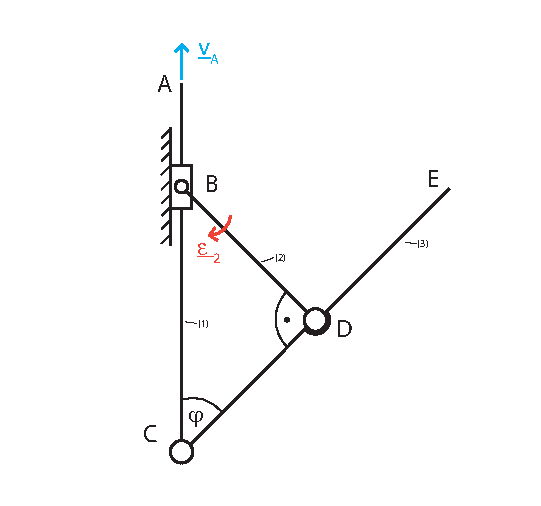
\includegraphics[width=.45\paperwidth]{Képek/2009.10.13_A.pdf}
\end{center}

\vspace{2em}
\underline{\textbf{Feladatok:}}
\begin{enumerate}
    \item Rajzolja be az ábrába a (3) rúd pillanatnyi sebességpólusát! Határozza meg az E pont
    sebességét!
    \item Adja meg a (3) rúd szöggyorsulását és számitsa ki az A pont pillanatnyi
    \item Készítsen külön ábrát és jelleghelyesen adja meg a (3) rúd gyorsuláspólusának helyét!
    \item Vizsgálja az (1) rúd C pontjának mozgását a (2) rúdhoz képest! Készitsen külön ábrát és
    jelleghelyesen rajzolja be a C pont szállitó-és relativ sebességét, valamint a C pont
    Coriolis gyorsulását!
\end{enumerate}

%------------------------------------------------------------------------------------------
%------------------------------------------------------------------------------------------
%------------------------------------------------------------------------------------------

\newpage

\setstretch{1.5}
\begin{center}
    \textbf{\LARGE{Dinamika}}\\
    1. Zárthelyi\\
    2009.10.13. B csoport
\end{center}
Az ábrán vazolt mechanizmus egy rögzitett csúszkából és három rúdból áll. A rudak egymáshoz
esuklósan kapcsolódnak. A (1) és (2) jelü rudak egymással pillanatnyilag derékszöget zárnak be.
Ismert a (3) rúd E végpontjának pillanatnyi sebessége és a (2) rúd pillanatnyi szöggyorsulása.\\\\
\underline{\textbf{Adatok:}}\\
$l_2 = 0,14 [m]$\\
$l_3 = 0,28 [m]$\\
$\varphi = 45 [^\circ]$\\
$v_E = 2 \left[\dfrac{m}{s}\right]$\\
$\varepsilon_2 = 20 \left[\dfrac{rad}{sec^2}\right]$
\begin{center}
    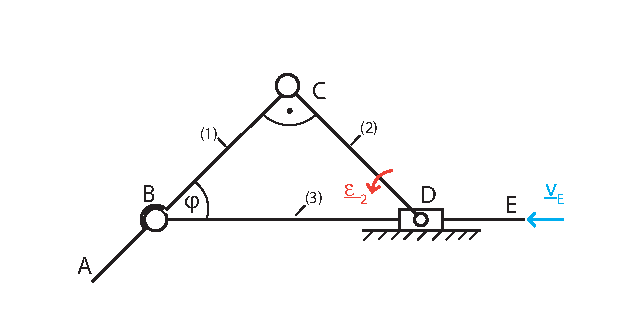
\includegraphics[width=.65\paperwidth]{Képek/2009.10.13_B.pdf}
\end{center}

\vspace{2em}
\underline{\textbf{Feladatok:}}
\begin{enumerate}
    \item Rajzolja be az brába az (1) rúd pillanatnyi sebességpólusát! Határozza meg az A pont
    sebességét!
    \item Adja meg az (1) rúd szöggyorsulását és számitsa ki az E pont pillanatnyi gyorsulását!
    \item Készitsen külön ábrát és jelleghelyesen adja meg az (1) rúd gyorsuláspólusának helyét!
    \item Vizsgálja a (3) rúd B pontjának mozgását a (2) rúdhoz képest! Készitsen külön ábrát és
    jelleghelyesen rajzolja be a B pont szállitó- és relativ sebességét, valamint a B pont Coriolis gyorsulasat!
\end{enumerate}
%------------------------------------------------------------------------------------------
%------------------------------------------------------------------------------------------
%------------------------------------------------------------------------------------------
\newpage

\setstretch{1.5}
\begin{center}
    \textbf{\LARGE{Dinamika}}\\
    1. Zárthelyi\\
    2010.10.11. B csoport
\end{center}
Az ábrán vázolt kétcsuklós robotkar C végpontja a szaggatott vonallal jelzett egyenes pályán mozog. A pályához tartozó befutási \\\\
\underline{\textbf{Adatok:}}\\
$l_2 = 0,14 [m]$\\
$l_3 = 0,28 [m]$\\
$\varphi = 45 [^\circ]$\\
$v_E = 2 \left[\dfrac{m}{s}\right]$\\
$\varepsilon_2 = 20 \left[\dfrac{rad}{sec^2}\right]$
\begin{center}
    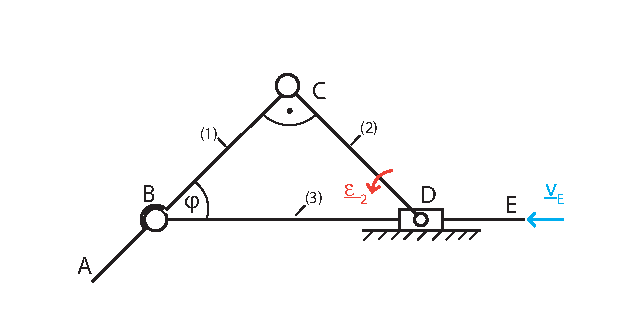
\includegraphics[width=.65\paperwidth]{Képek/2009.10.13_B.pdf}
\end{center}

\vspace{2em}
\underline{\textbf{Feladatok:}}
\begin{enumerate}
    \item Rajzolja be az brába az (1) rúd pillanatnyi sebességpólusát! Határozza meg az A pont
    sebességét!
    \item Adja meg az (1) rúd szöggyorsulását és számitsa ki az E pont pillanatnyi gyorsulását!
    \item Készitsen külön ábrát és jelleghelyesen adja meg az (1) rúd gyorsuláspólusának helyét!
    \item Vizsgálja a (3) rúd B pontjának mozgását a (2) rúdhoz képest! Készitsen külön ábrát és
    jelleghelyesen rajzolja be a B pont szállitó- és relativ sebességét, valamint a B pont Coriolis gyorsulasat!
\end{enumerate}
\end{document}